% preamble-exam-zh.tex — 极简讲解页共享 preamble
% 目标：复刻「题目独立、提示轻框、路线箭头、主体双栏、答案轻收束」的讲义风格。

\documentclass{exam-zh}

% ---------- 基础配置 ----------
\examsetup{
  page/size = a4paper,
  page/show-head = false,
  page/show-foot = false,
  sealline/show = false,
  font = none,
  math-font = none,
}

% ---------- 包 ----------
\usepackage{geometry}
\geometry{top=10mm,bottom=14mm,left=12mm,right=10mm}
\AtBeginDocument{\newgeometry{top=10mm,bottom=14mm,left=12mm,right=10mm}}

\usepackage{xcolor}
\usepackage{needspace}
\usepackage{enumitem}
\usepackage{array}
\usepackage{tabularx}
\usepackage{tcolorbox}
\tcbuselibrary{skins,breakable}
\usepackage{paracol}
\usepackage{graphicx}

% ---------- 打印/屏幕颜色切换 ----------
% 用法：\documentclass[monochrome]{exam-zh} 可降级为灰度。
% 注意：不要使用 \if@xxx 放在 makeatother 外部；这里改成普通条件名。
\newif\ifeduprintcolor
\eduprintcolortrue
\makeatletter
\@ifclasswith{exam-zh}{monochrome}{\eduprintcolorfalse}{}
\makeatother

% ---------- 语义颜色 ----------
\ifeduprintcolor
  \definecolor{edu-blue}{RGB}{31,62,126}
  \definecolor{edu-blue-soft}{RGB}{232,238,250}
  \definecolor{edu-blue-bg}{RGB}{248,250,254}
  \definecolor{edu-ink}{RGB}{30,35,45}
  \definecolor{edu-muted}{RGB}{118,124,136}
  \definecolor{edu-line}{RGB}{209,218,235}
  \definecolor{edu-soft-bg}{RGB}{250,251,253}
  \definecolor{edu-red}{RGB}{168,58,58}
  \definecolor{edu-red-bg}{RGB}{255,247,245}
\else
  \definecolor{edu-blue}{gray}{0.15}
  \definecolor{edu-blue-soft}{gray}{0.90}
  \definecolor{edu-blue-bg}{gray}{0.98}
  \definecolor{edu-ink}{gray}{0.10}
  \definecolor{edu-muted}{gray}{0.45}
  \definecolor{edu-line}{gray}{0.82}
  \definecolor{edu-soft-bg}{gray}{0.97}
  \definecolor{edu-red}{gray}{0.28}
  \definecolor{edu-red-bg}{gray}{0.97}
\fi
\colorlet{edu-diagram-muted}{edu-muted}

% ---------- 全局排版 ----------
\setlength{\parindent}{0pt}
\setlength{\parskip}{0pt}
\linespread{1.16}
\renewcommand{\arraystretch}{1.15}

% ctex 通常提供 \kaishu；这里用它做教师旁白感。
\newcommand{\edukai}{\kaishu}

% ---------- 顶部元信息 ----------
\newcommand{\eduTopBar}[2]{%
  \noindent
  \begin{tabularx}{\linewidth}{@{}Xr@{}}
    {\color{edu-blue}\bfseries #1} &
    {\color{edu-blue}\bfseries #2}
  \end{tabularx}
  \vspace{8mm}
}

% ---------- 轻标题体系 ----------
% 只有真正的大结构才用它；不要给提示/路线滥用标题。
\newcommand{\eduSectionTitle}[1]{%
  \needspace{5\baselineskip}%
  \vspace{2mm}
  {\color{edu-blue}\bfseries\large #1}\par
  \vspace{3mm}
}

\newcommand{\eduSubTitle}[1]{%
  \needspace{4\baselineskip}%
  \vspace{1mm}
  {\color{edu-blue}\bfseries #1}\par
  \vspace{1mm}
}

% ---------- 小问题干：复用 exam (1)(2)(3) 格式 ----------
\newenvironment{eduSubQuestionItem}[1]{%
  \needspace{4\baselineskip}%
  \vspace{2mm}
  \par\noindent
  \hangindent=8mm\hangafter=1
  {\color{edu-blue}\bfseries #1}\enspace
  \begingroup
  \color{edu-ink}
}{%
  \endgroup
  \par
  \vspace{3mm}
}

% ---------- 辅助信息条（解题流程/关键想法/思考）楷体 ----------
\newenvironment{eduAuxItem}[1]{%
  \needspace{4\baselineskip}%
  \vspace{2mm}
  \par\noindent
  \hangindent=8mm\hangafter=1
  {\color{edu-blue}\edukai $\triangleright$~#1}\enspace
  \begingroup
  \color{edu-ink}
  \edukai
}{%
  \endgroup
  \par
  \vspace{4mm}
}

\newcommand{\eduColumnTitle}[2]{%
  {\color{edu-blue}\bfseries #1\hspace{1.5mm}#2}\par
  \vspace{2.5mm}
}

% ---------- 图标：不用外部 icon 字体，保证可移植 ----------
\newcommand{\eduIconBulb}{\(\circ\)}
\newcommand{\eduIconBook}{\(\square\)}
\newcommand{\eduIconCheck}{\(\checkmark\)}
\newcommand{\eduIconPin}{\(\diamond\)}
\newcommand{\eduIconNote}{\(\triangleright\)}

% ---------- 题目区 ----------
% 题目区是页面入口：弱标签 + 一条长蓝线 + 大题干。
\newenvironment{eduProblemBlock}[1][题目]{%
  \needspace{8\baselineskip}
  {\small\color{edu-muted}#1}\par
  \vspace{1.5mm}
  {\color{edu-blue}\hrule height 0.55pt}
  \vspace{4.5mm}
  \begingroup
  \color{edu-ink}
  \large
  \setlength{\parskip}{2.2mm}
  \linespread{1.20}\selectfont
}{%
  \par
  \endgroup
  \vspace{6mm}
}

\newenvironment{eduSubQuestions}{%
  \begin{enumerate}[
    label=(\arabic*),
    leftmargin=8mm,
    itemsep=2.0mm,
    topsep=2.0mm,
    parsep=0pt
  ]
}{%
  \end{enumerate}
}

% ---------- 读题提示：轻框，不做同级标题 ----------
\newtcolorbox{eduReadTipBox}{
  enhanced,
  breakable,
  colback=white,
  colframe=edu-blue!45,
  boxrule=0.45pt,
  arc=1.6mm,
  left=10mm,
  right=4mm,
  top=5mm,
  bottom=5mm,
  before skip=1mm,
  after skip=7mm,
  fontupper=\edukai\normalsize,
  colupper=edu-ink,
  overlay={
    \node[anchor=north west, text=edu-blue] at ([xshift=3.2mm,yshift=-3.2mm]frame.north west)
    {\small\eduIconNote};
  }
}

\newenvironment{eduTipList}{%
  \begin{itemize}[
    label=\textbullet,
    leftmargin=5mm,
    itemsep=1.2mm,
    topsep=0pt,
    parsep=0pt
  ]
}{%
  \end{itemize}
}

% ---------- 解题路线：虚线框 + 文字箭头 ----------
\newenvironment{eduRouteFlow}{%
  \needspace{4\baselineskip}%
  \vspace{1mm}
  \begin{center}
  \normalsize
}{%
  \end{center}
  \vspace{7mm}
}
\newcommand{\eduRouteStep}[1]{%
  {\color{edu-ink}#1}%
}
\newcommand{\eduRouteArrow}{%
  \;$\boldsymbol{\to}$\;%
}

% ---------- 主体讲解：使用 paracol 实现跨页自适应双栏 ----------
\newenvironment{eduDualExplain}{%
  \needspace{6\baselineskip}% 防止标题孤行
  \columnratio{0.26, 0.74}%
  \setlength{\columnsep}{8mm}%
  \columnseprule=0.45pt%
  \colseprulecolor{edu-blue}%
  \begin{paracol}{2}% 开启双栏
}{%
  \end{paracol}% 结束双栏
  \vspace{5mm}
}

\newenvironment{eduExplainLeft}{%
  \setlength{\linewidth}{\columnwidth}%
  \hsize=\columnwidth
  \normalsize\color{edu-ink}%
}{%
  \switchcolumn
}

\newcommand{\eduColumnDivider}{}

\newenvironment{eduExplainRight}{%
  \setlength{\linewidth}{\columnwidth}%
  \hsize=\columnwidth
  \normalsize\color{edu-ink}%
}{%
}

\newtcolorbox{eduSideHintBox}[1]{
  enhanced,
  breakable,
  colback=edu-blue-bg,
  colframe=edu-line,
  boxrule=0.35pt,
  borderline west={1.5pt}{0pt}{edu-blue},
  arc=0.8mm,
  left=2.4mm,
  right=2.4mm,
  top=2mm,
  bottom=2mm,
  before skip=1mm,
  after skip=1.5mm,
  title={\color{edu-blue}\bfseries\small #1},
  coltitle=edu-blue,
  attach title to upper={\par\vspace{0.7mm}},
  fontupper=\small
}

\newtcolorbox{eduSideMistakeBox}[1]{
  enhanced,
  breakable,
  colback=edu-red-bg,
  colframe=edu-red!35,
  boxrule=0.35pt,
  borderline west={1.5pt}{0pt}{edu-red},
  arc=0.8mm,
  left=2.4mm,
  right=2.4mm,
  top=2mm,
  bottom=2mm,
  before skip=1mm,
  after skip=1.5mm,
  title={\color{edu-red}\bfseries\small #1},
  coltitle=edu-red,
  attach title to upper={\par\vspace{0.7mm}},
  fontupper=\small
}

\newtcolorbox{eduSideNoteBox}[1]{
  enhanced,
  breakable,
  colback=edu-soft-bg,
  colframe=edu-line,
  boxrule=0.35pt,
  borderline west={1.5pt}{0pt}{edu-muted},
  arc=0.8mm,
  left=2.4mm,
  right=2.4mm,
  top=2mm,
  bottom=2mm,
  before skip=1mm,
  after skip=1.5mm,
  title={\color{edu-muted}\bfseries\small #1},
  coltitle=edu-muted,
  attach title to upper={\par\vspace{0.7mm}},
  fontupper=\small
}

\newcommand{\eduSideHint}[2]{%
  \begin{eduSideHintBox}{#1}#2\end{eduSideHintBox}%
}
\newcommand{\eduSideMistake}[2]{%
  \begin{eduSideMistakeBox}{#1}#2\end{eduSideMistakeBox}%
}
\newcommand{\eduSideNote}[2]{%
  \begin{eduSideNoteBox}{#1}#2\end{eduSideNoteBox}%
}

\newcommand{\eduExplainStep}[3]{%
  \needspace{3\baselineskip}%
  \vspace{1.2mm}%
  {\color{edu-blue}\bfseries step#1.\enspace #2}\par
  \vspace{0.8mm}%
  \begingroup
  \color{edu-ink}#3\par
  \endgroup
  \vspace{2.2mm}%
}

\newenvironment{eduNumberList}{%
  \begin{enumerate}[
    label=\arabic*.,
    leftmargin=6mm,
    itemsep=4.8mm,
    topsep=0pt,
    parsep=0pt
  ]
}{%
  \end{enumerate}
}

\newenvironment{eduBulletList}{%
  \begin{itemize}[
    label=\textbullet,
    leftmargin=5mm,
    itemsep=1.2mm,
    topsep=0pt,
    parsep=0pt
  ]
}{%
  \end{itemize}
}

% ---------- 底部双栏：答案 + 方法提醒 ----------
\newenvironment{eduBottomGrid}{%
  \columnratio{0.32, 0.68}%
  \setlength{\columnsep}{11mm}%
  \columnseprule=0pt%
  \begin{paracol}{2}%
}{%
  \end{paracol}%
}

\newenvironment{eduSummaryLeft}{%
}{%
}

\newcommand{\eduSummaryDivider}{%
  \switchcolumn
}

\newenvironment{eduSummaryRight}{%
}{%
}

% ---------- 答案/方法提醒：轻量收束 ----------
\newtcolorbox{eduSummaryBlock}[2]{
  enhanced,
  breakable,
  colback=edu-blue-bg,
  colframe=edu-line,
  boxrule=0.45pt,
  arc=1.2mm,
  left=3.5mm,
  right=3.5mm,
  top=3mm,
  bottom=3mm,
  before skip=1mm,
  after skip=2.5mm,
  title={\color{edu-blue}\bfseries #1\hspace{1.5mm}#2},
  coltitle=edu-blue,
  attach title to upper={\par\vspace{1.5mm}},
  fontupper=\normalsize
}

% ---------- 例题单栏解答卡片 ----------
\newtcolorbox{eduSolutionBox}[1]{
  enhanced,
  breakable,
  colback=white,
  colframe=edu-blue!40,
  boxrule=0.55pt,
  arc=1.2mm,
  left=4mm,
  right=4mm,
  top=3.5mm,
  bottom=3.5mm,
  before skip=2mm,
  after skip=3mm,
  title={\color{edu-blue}\bfseries \eduIconBook\hspace{1.5mm}#1},
  coltitle=edu-blue,
  attach title to upper={\par\vspace{1.5mm}},
  fontupper=\normalsize
}

% ---------- 变式训练：完整题目 + 学生留白 ----------
\newtcolorbox{eduVariationTraining}[1]{
  enhanced,
  breakable,
  colback=white,
  colframe=edu-blue!45,
  boxrule=0.5pt,
  borderline west={1.8pt}{0pt}{edu-blue},
  arc=1.2mm,
  left=4mm,
  right=4mm,
  top=3.2mm,
  bottom=3.2mm,
  before skip=2mm,
  after skip=4mm,
  title={\color{edu-blue}\bfseries #1},
  coltitle=edu-blue,
  attach title to upper={\par\vspace{1.8mm}},
  fontupper=\normalsize,
  colupper=edu-ink
}

\newenvironment{eduPlainList}{%
  \begin{enumerate}[
    label=(\arabic*),
    leftmargin=7mm,
    itemsep=1.2mm,
    topsep=0pt,
    parsep=0pt
  ]
}{%
  \end{enumerate}
}

% ---------- 兼容旧 block 的轻量盒子 ----------
\newtcolorbox{eduSoftBox}{
  enhanced,
  breakable,
  colback=edu-soft-bg,
  colframe=edu-line,
  boxrule=0.35pt,
  arc=1mm,
  left=3mm,
  right=3mm,
  top=2mm,
  bottom=2mm,
  before skip=1mm,
  after skip=2mm,
  fontupper=\small
}

\newtcolorbox{eduMistakeBox}{
  enhanced,
  breakable,
  colback=edu-red-bg,
  colframe=edu-red!40,
  boxrule=0.35pt,
  arc=1mm,
  left=3mm,
  right=3mm,
  top=2.5mm,
  bottom=2.5mm,
  before skip=1mm,
  after skip=2mm,
  fontupper=\normalsize
}

\newtcolorbox{eduLegacySolution}{
  enhanced,
  breakable,
  colback=edu-soft-bg,
  colframe=edu-line,
  boxrule=0.35pt,
  arc=1mm,
  left=3mm,
  right=3mm,
  top=2mm,
  bottom=2mm,
  before skip=-2mm,
  after skip=4mm,
  fontupper=\small
}

\newtcolorbox{eduTeacherNote}{
  enhanced,
  breakable,
  colback=edu-soft-bg,
  colframe=edu-line,
  boxrule=0pt,
  borderline west={1.5pt}{0pt}{edu-muted},
  left=2.5mm,
  right=2.5mm,
  top=2mm,
  bottom=2mm,
  before skip=1mm,
  after skip=2mm,
  fontupper=\footnotesize,
  colupper=edu-muted
}

% ---------- 答题区 ----------
\newcommand{\answerarea}[1][40mm]{%
  \vspace{3mm}%
  \begin{tcolorbox}[
    enhanced,
    breakable,
    colback=white,
    colframe=edu-line,
    boxrule=0.55pt,
    arc=0.8mm,
    height=#1,
    valign=top,
  ]
  \end{tcolorbox}%
}

\newcommand{\diagramcolfigure}[3]{%
  \begin{minipage}[t]{#2}
    \vspace{0pt}\centering
    \includegraphics[width=\linewidth]{\detokenize{#1}}
    \if\relax\detokenize{#3}\relax\else
      \par\vspace{1mm}{\scriptsize\color{edu-diagram-muted}#3}
    \fi
  \end{minipage}%
}

\newcommand{\diagramrowitem}[4]{%
  \begin{minipage}[t]{#2}
    \vspace{0pt}\centering
    \includegraphics[width=\linewidth]{\detokenize{#1}}
    \if\relax\detokenize{#3}\relax\else
      \par\vspace{1mm}{\scriptsize\bfseries #3}
    \fi
    \if\relax\detokenize{#4}\relax\else
      \par\vspace{0.5mm}{\scriptsize\color{edu-diagram-muted}#4}
    \fi
  \end{minipage}%
}

\newcommand{\answerareawithdiagramcol}[4]{%
  \vspace{3mm}%
  \begin{tcolorbox}[
    enhanced,
    breakable,
    colback=white,
    colframe=edu-line,
    boxrule=0.55pt,
    arc=0.8mm,
    height=#1,
    valign=top,
  ]
  \begin{minipage}[t]{\dimexpr\linewidth-#3-6mm\relax}
    \vspace{0pt}
  \end{minipage}\hfill
  \diagramcolfigure{#2}{#3}{#4}
  \end{tcolorbox}%
}

\newcommand{\answerareawithdiagram}[4]{%
  \answerareawithdiagramcol{#1}{#2}{#3}{#4}%
}

\examsetup{
  question/show-answer = true,
  fillin/show-answer = true,
  solution/show-solution = show-stay,
}

\begin{document}

\eduSectionTitle{模型：角平分线和平行线推出等腰}


\begin{eduSolutionBox}{核心结论：角平分、平行线、翻折都在制造等角}
  \begingroup
  \setlength{\parskip}{2.5mm}
角平分线给出一组相等角。\par
平行线给出另一组相等角。\par
翻折题中，折痕两侧的对应角相等；常常等价于出现一条角平分线。\par
两组角合在一起，推出某个三角形有两个角相等。\par
两角相等，则所对的边相等。\par
  \endgroup
\end{eduSolutionBox}




\begin{eduProblemBlock}[例题 1]
如图，在矩形 $ABCD$ 中，$BE$ 平分 $\angle ABC$，交 $AD$ 于点 $E$，连接 $CE$。若 $AB=5$，$BC=8$，求 $CE$ 的长。
\begin{center}
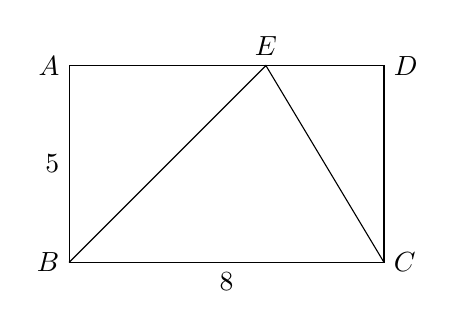
\begin{tikzpicture}[scale=0.5]
  \coordinate (A) at (0,5); \coordinate (B) at (0,0);
  \coordinate (C) at (8,0); \coordinate (D) at (8,5);
  \coordinate (E) at (5,5);
  \draw (A)--(B)--(C)--(D)--cycle;
  \draw (B)--(E)--(C);
  \node[left] at (A){$A$}; \node[left] at (B){$B$};
  \node[right] at (C){$C$}; \node[right] at (D){$D$}; \node[above] at (E){$E$};
  \node[left] at (0,2.5){$5$}; \node[below] at (4,0){$8$};
\end{tikzpicture}
\end{center}

\end{eduProblemBlock}





\begin{eduAuxItem}{思路导航}
证明等腰$\;\to\;$求 $CE$\end{eduAuxItem}




\begin{eduSubQuestionItem}{例题 1}
求 $CE$。\end{eduSubQuestionItem}

\begin{eduDualExplain}
  \begin{eduExplainLeft}
    \eduColumnTitle{\eduIconBulb}{小贴士}
        \eduSideMistake{等腰边别找错}{相等的是 $AE$ 和 $AB$，不是 $BE$。}
  \end{eduExplainLeft}

  \begin{eduExplainRight}
    \eduColumnTitle{\eduIconBook}{解答}
      \eduExplainStep{1}{证明等腰}{$BE$ 平分 $\angle ABC$，所以 $\angle ABE=\angle EBC$。又 $AD\parallel BC$，所以 $\angle AEB=\angle EBC$。因此 $\triangle ABE$ 是等腰三角形，$AE=AB=5$。}
      \eduExplainStep{2}{求 $CE$}{$DE=AD-AE=8-5=3$，$CD=5$，所以 $CE=\sqrt{5^2+3^2}=\sqrt{34}$。}
  \end{eduExplainRight}
\end{eduDualExplain}




\begin{eduProblemBlock}[例题 2]
如图，在矩形 $ABCD$ 中，$AB=6$，$BC=8$。沿对角线 $AC$ 翻折，使点 $B$ 落在点 $B'$ 处，线段 $CB'$ 交 $AD$ 于点 $E$。求 $AE$ 的长。
\begin{center}
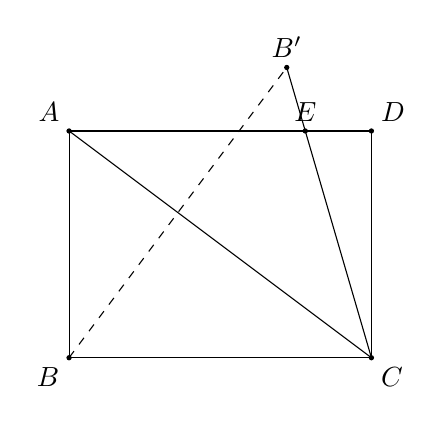
\begin{tikzpicture}[scale=0.48]
  \coordinate (A) at (0,6); \coordinate (B) at (0,0);
  \coordinate (C) at (8,0); \coordinate (D) at (8,6);
  \coordinate (E) at (6.25,6); \coordinate (Bp) at (5.76,7.68);
  \draw (A)--(B)--(C)--(D)--cycle;
  \draw (A)--(C);
  \draw[dashed] (B)--(Bp);
  \draw (C)--(Bp);
  \fill (A) circle(2pt) node[above left]{$A$};
  \fill (B) circle(2pt) node[below left]{$B$};
  \fill (C) circle(2pt) node[below right]{$C$};
  \fill (D) circle(2pt) node[above right]{$D$};
  \fill (E) circle(2pt) node[above]{$E$};
  \fill (Bp) circle(2pt) node[above]{$B'$};
\end{tikzpicture}
\end{center}

\end{eduProblemBlock}





\begin{eduAuxItem}{思路导航}
翻折和平行线给等角$\;\to\;$得到等腰三角形$\;\to\;$列方程求 $AE$\end{eduAuxItem}




\begin{eduSubQuestionItem}{例题 2}
用翻折中的等角关系求 $AE$。\end{eduSubQuestionItem}

\begin{eduDualExplain}
  \begin{eduExplainLeft}
    \eduColumnTitle{\eduIconBulb}{小贴士}
        \eduSideHint{翻折看角}{折过去的线段和原线段对应，角也对应相等；再用矩形的平行边把角搬到 $\triangle AEC$。}
  \end{eduExplainLeft}

  \begin{eduExplainRight}
    \eduColumnTitle{\eduIconBook}{解答}
      \eduExplainStep{1}{翻折和平行线给等角}{沿 $AC$ 翻折，$CB$ 的对应线段为 $CB'$，所以 $\angle BCA=\angle ACB'$。又 $AD\parallel BC$，所以 $\angle EAC=\angle BCA$。因此 $\angle EAC=\angle ACE$。}
      \eduExplainStep{2}{得到等腰三角形}{$\triangle AEC$ 中两个底角相等，所以 $AE=CE$。}
      \eduExplainStep{3}{列方程求 $AE$}{设 $AE=x$，则 $DE=8-x$，$CD=6$。由 $CE=AE$，得 $x^2=(8-x)^2+6^2$，解得 $x=\dfrac{25}{4}$。}
  \end{eduExplainRight}
\end{eduDualExplain}




\begin{eduProblemBlock}[例题 3]
如图，在正方形 $ABCD$ 中，点 $E$ 是 $CD$ 的中点，$BF$ 平分 $\angle ABE$，交 $AD$ 于点 $F$。以 $B$ 为原点，以 $BC$ 所在直线为 $x$ 轴，以 $BA$ 所在直线为 $y$ 轴建立坐标系。若 $E(2,1)$，求点 $D$ 和点 $F$ 的坐标。
\begin{center}
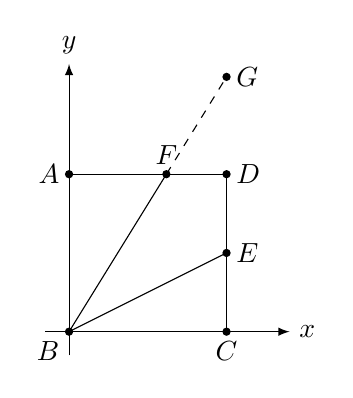
\begin{tikzpicture}[scale=1.0,>=latex]
  \draw[->] (-0.3,0)--(2.8,0) node[right]{$x$};
  \draw[->] (0,-0.3)--(0,3.4) node[above]{$y$};
  \coordinate (B) at (0,0); \coordinate (C) at (2,0);
  \coordinate (D) at (2,2); \coordinate (A) at (0,2);
  \coordinate (E) at (2,1); \coordinate (G) at (2,3.236);
  \coordinate (F) at (1.236,2);
  \draw (A)--(B)--(C)--(D)--cycle;
  \draw (B)--(E); \draw (B)--(F); \draw[dashed] (F)--(G);
  \foreach \p/\pos in {A/left,B/below left,C/below,D/right,E/right,F/above,G/right}
    \fill (\p) circle(1.5pt) node[\pos]{$\p$};
\end{tikzpicture}
\end{center}

\end{eduProblemBlock}





\begin{eduAuxItem}{思路导航}
确定正方形$\;\to\;$延长得到等腰$\;\to\;$求 $F$\end{eduAuxItem}




\begin{eduSubQuestionItem}{例题 3}
求 $D,F$ 的坐标。\end{eduSubQuestionItem}

\begin{eduDualExplain}
  \begin{eduExplainLeft}
    \eduColumnTitle{\eduIconBulb}{小贴士}
        \eduSideHint{为什么延长}{延长到 $CD$ 所在直线后，才能用 $AB\parallel GE$ 搬角。}
  \end{eduExplainLeft}

  \begin{eduExplainRight}
    \eduColumnTitle{\eduIconBook}{解答}
      \eduExplainStep{1}{确定正方形}{$E$ 是 $CD$ 中点且 $E(2,1)$，所以正方形边长为 $2$，$D(2,2)$。}
      \eduExplainStep{2}{延长得到等腰}{延长 $BF$ 交 $CD$ 延长线于 $G$。由 $AB\parallel GE$ 和角平分线，得 $\triangle BGE$ 为等腰三角形，$GE=BE=\sqrt5$。}
      \eduExplainStep{3}{求 $F$}{$G(2,1+\sqrt5)$，直线 $BG:y=\dfrac{1+\sqrt5}{2}x$。令 $y=2$，得 $x=\sqrt5-1$，所以 $F(\sqrt5-1,2)$。}
  \end{eduExplainRight}
\end{eduDualExplain}




\end{document}
